%-------------------------------------------------------------------------
\begin{figure}[t]
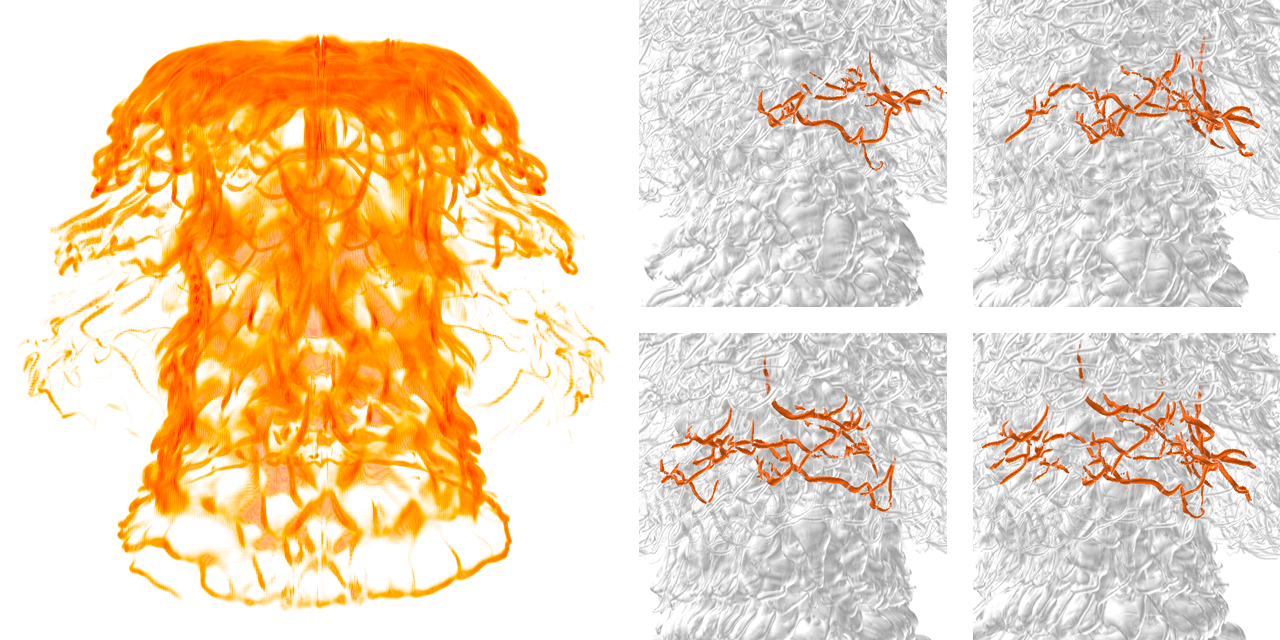
\includegraphics[width=1.0\linewidth]{combustion_ft.png}
\caption{Left: The volume rendering of a single time step of the combustion data set; Right: Selected features of interest extracted and tracked overtime.}
\label{fig:combustion-labeled}
\end{figure}

\begin{figure}[t]
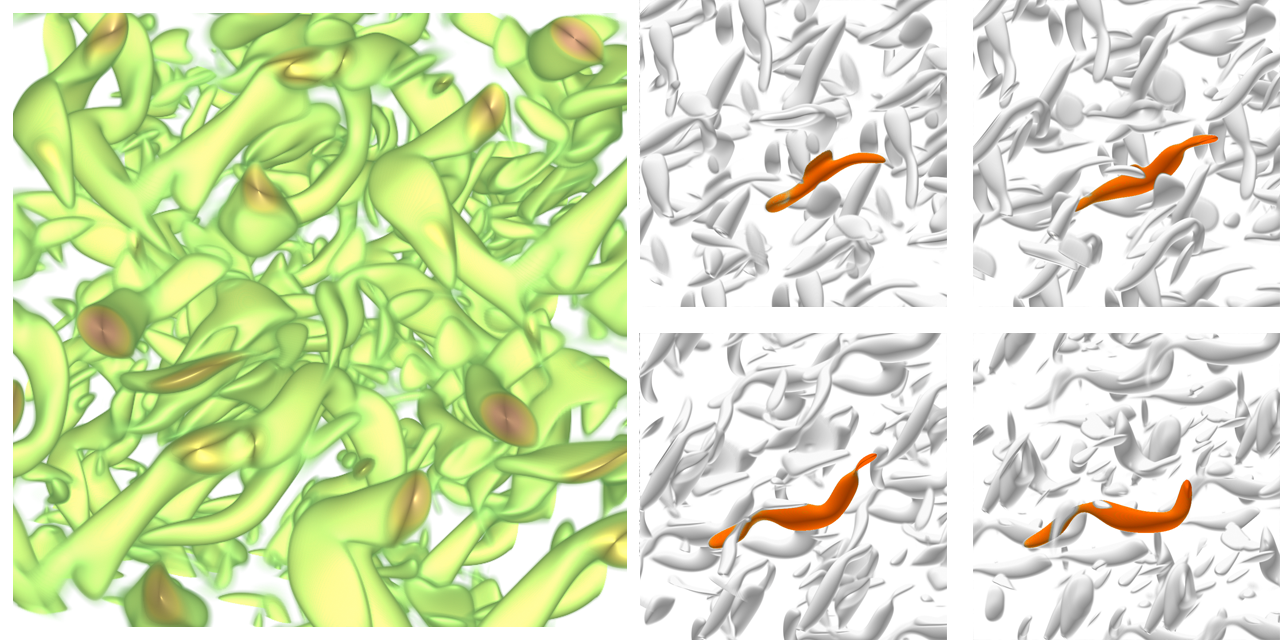
\includegraphics[width=1.0\linewidth]{vorts_ft.png}
\caption{Left: The volume rendering of a single time step of the vortex data set; Right: Selected features of interest extracted and tracked overtime.}
\label{fig:vorts-tracking-result}
\end{figure}
%-------------------------------------------------------------------------

\section{Results}

We test our feature extraction and tracking algorithm using the NERSC Hopper cluster on two datasets. A 400 time steps $256^{3}$ vortex data set obtained from a combustion solver that can simulate turbulent flames, and a 100 time steps $1024^{3}$ vortex data set synthesized from the $128^{3}$ volume data set used in the other works~\cite{Silver1997, Ji2003, Ji2006}. In the combustion data set, each voxel contains the magnitude value of vorticity derived from velocity using a curl operator. As time evolves, vortical features may vary from small amassed blob features to long curly features that span over large portion of the volume. Figures~\ref{fig:combustion-labeled} and \ref{fig:vorts-tracking-result} show the examples of identified and tracked features in these two data sets, which match the non-parallelized tracking results. We ignore the I/O cost and only focus on the computation time in our study.

\textbf{Time for extracting features ($T_{extract}$): } 
Because we use region-growing based algorithm to extract features, given a fixed specification of feature, the computation time is determined by the size of the volume as well as the number of processors being used. Once the volume data and its partitioning, a.k.a. the size of each data block is determined, the computation time for extracting residing features remains approximately the same. In post-processing, the size of each data block decreases with the increasing number of processors, and hence so does the time spent on extracting features. As depicted in Figure~\ref{fig:feature-extraction}, $T_{extract}$ is approximately log-linear decreased as the number of processors increases.

\begin{figure}[t]
\centering
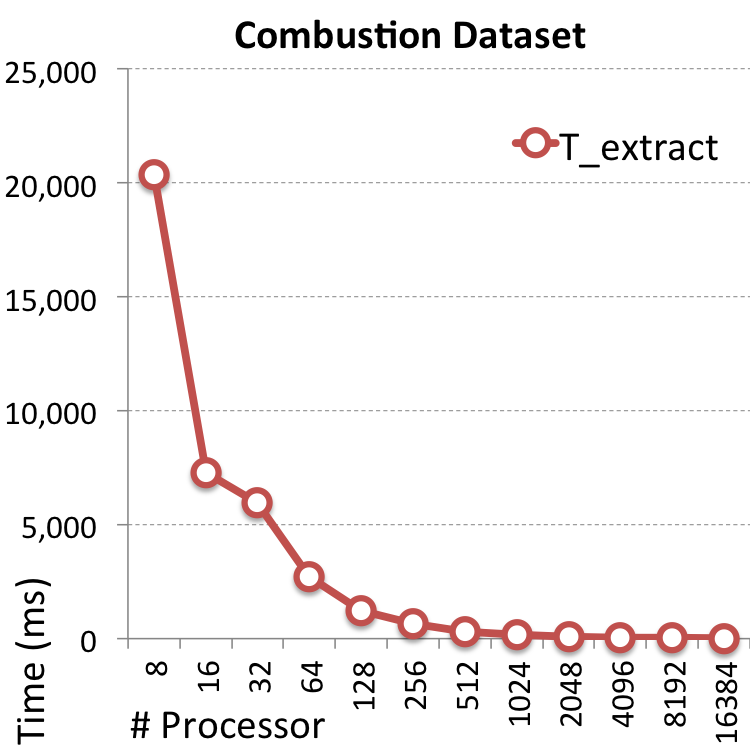
\includegraphics[width=0.49\linewidth]{combustion_t_extract.png}
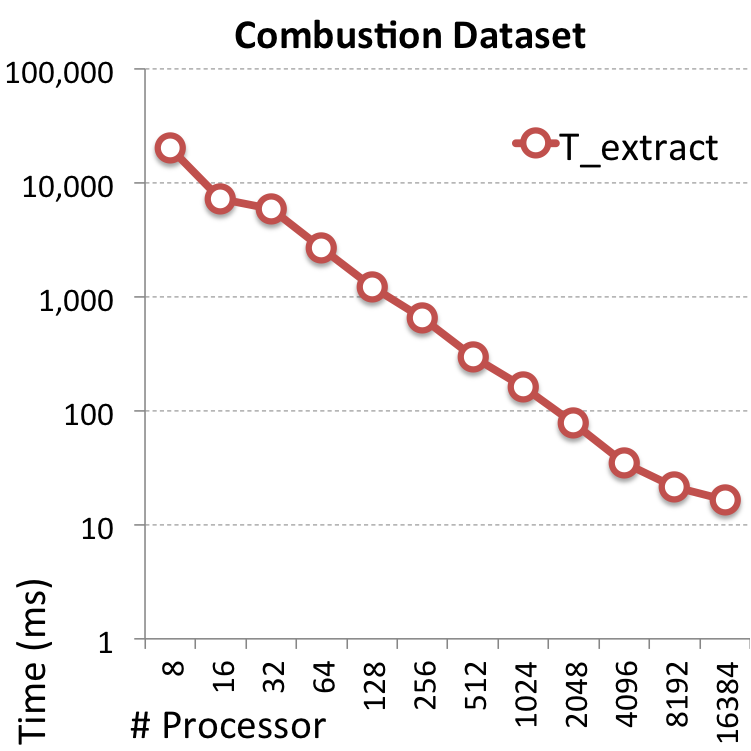
\includegraphics[width=0.49\linewidth]{combustion_t_extract_log.png}
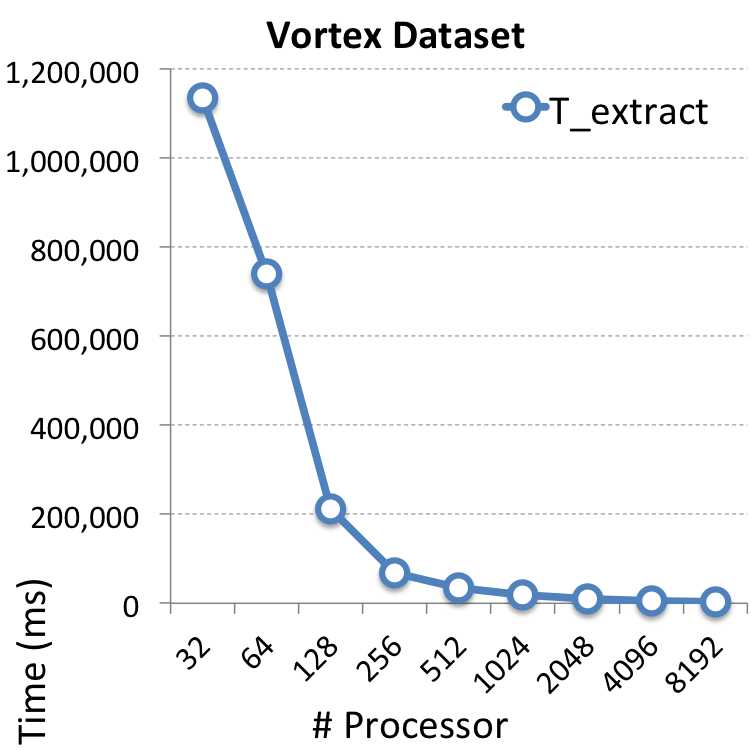
\includegraphics[width=0.49\linewidth]{vorts_t_extract.png}
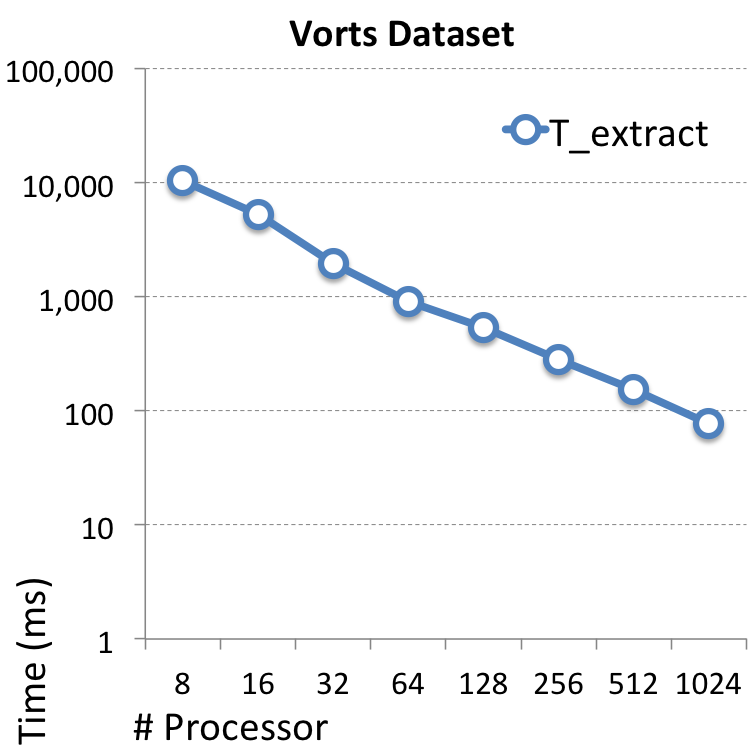
\includegraphics[width=0.49\linewidth]{vorts_t_extract_log.png}
\caption{Average computation cost per time step for feature extraction. The left two plots are shown in linear scale, and the right plots are shown in logarithmic scale. The speedup is nearly linear with the number of processors.}
\label{fig:feature-extraction}
\end{figure}

\textbf{Create Local Connectivity Tree ($T_{create}$): }
Despite the size of each data block, the computation cost for creating and updating local connectivity tree is dependent on the number of the features extracted within the original volume, or, more precisely, the number of features that touches the boundary surfaces of their residing data block. As shown in Figure~\ref{fig:create-local-graph}, similar to $T_{extract}$, $T_{create}$ decreases as the number of processors increases %in post-processing
, and as the number of feature-on-boundary decreases, accordingly. For both the combustion and vorticity data set, it takes an average of 0.1 seconds to create the local connectivity tree, approximately 0.5\% the time of $T_{extract}$ using the same amount of processors. The $T_{create}/T_{extract}$ ratio increases but does not succeed 1\% in our test, and hence, $T_{create}$ is not considered as a bottleneck. %

\begin{figure}[t]
\centering
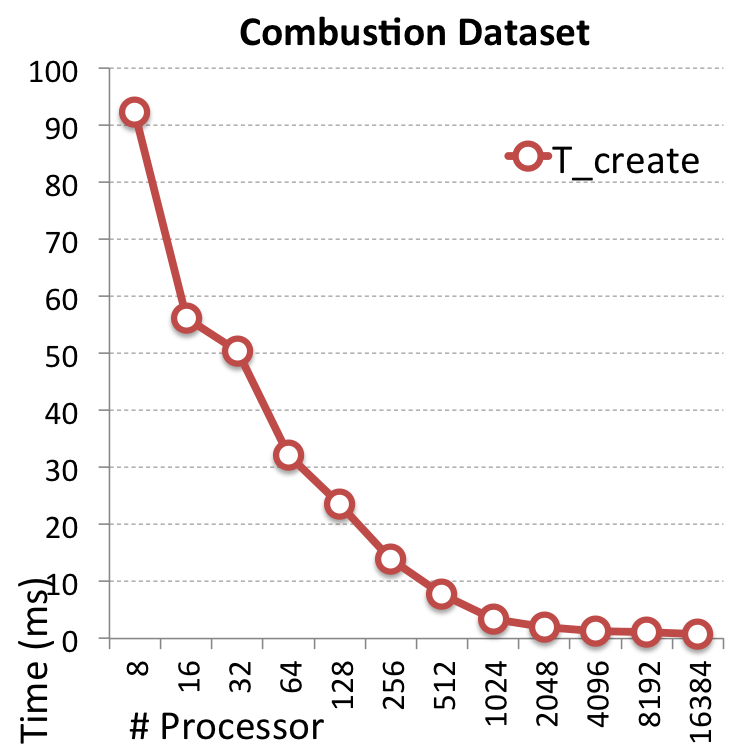
\includegraphics[width=0.49\linewidth]{combustion_t_create.png}
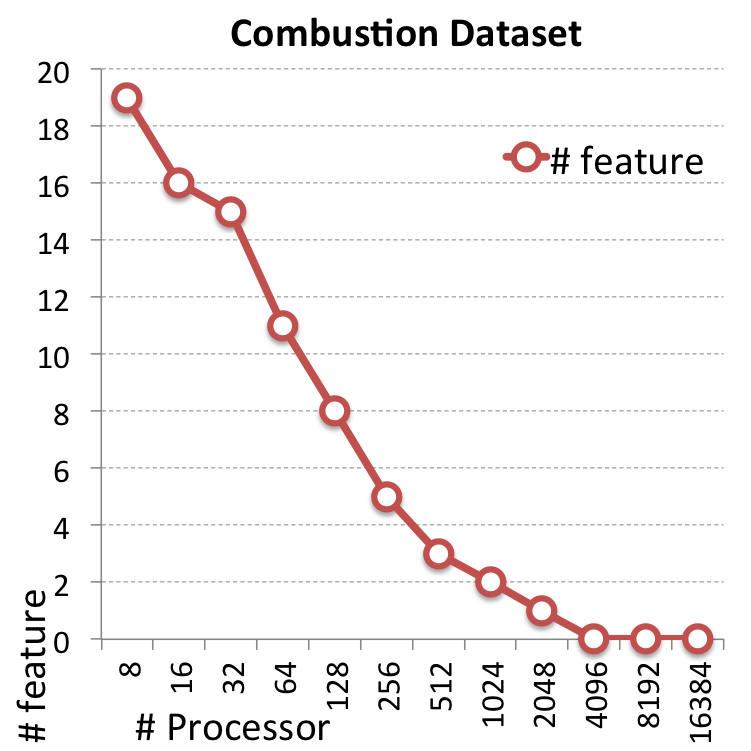
\includegraphics[width=0.49\linewidth]{combustion_num_feature.png}
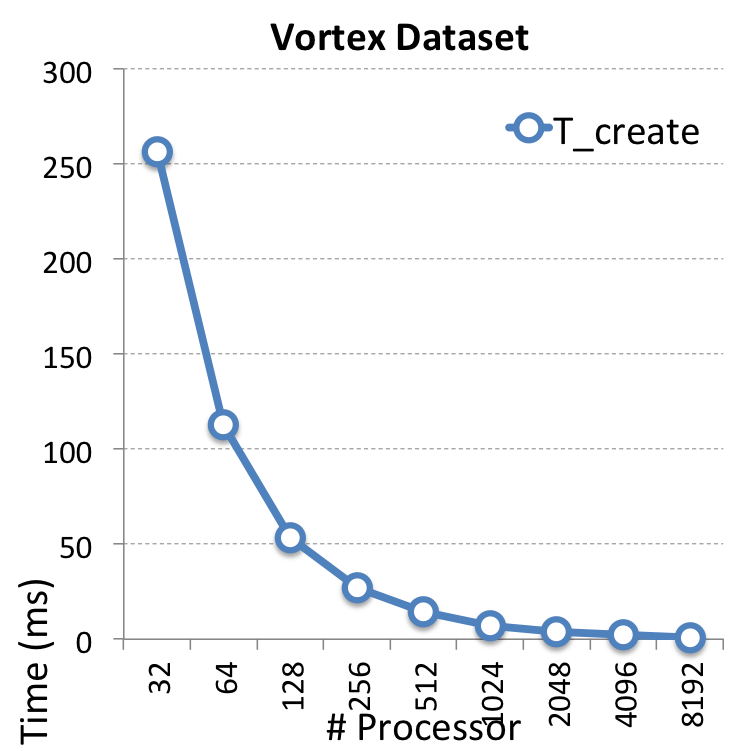
\includegraphics[width=0.49\linewidth]{vorts_t_create.png}
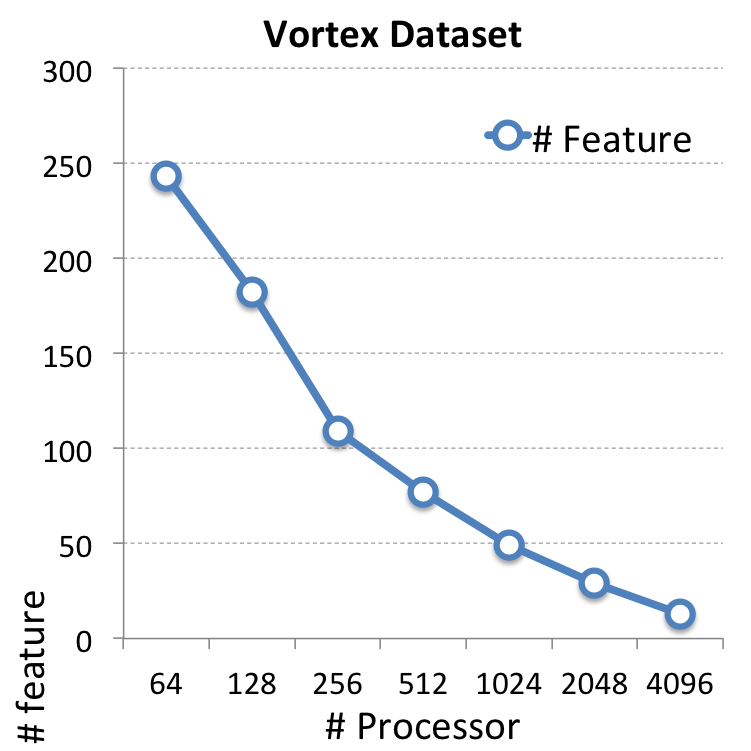
\includegraphics[width=0.49\linewidth]{vorts_num_feature.png}
\caption{Average computation cost per time step for creating local connectivity tree. The speedup is nearly linear with the number of processors. The time cost is approximately proportional to the number of features-on-boundary.}
\label{fig:create-local-graph}
\end{figure}

\begin{figure}[ht]
\centering
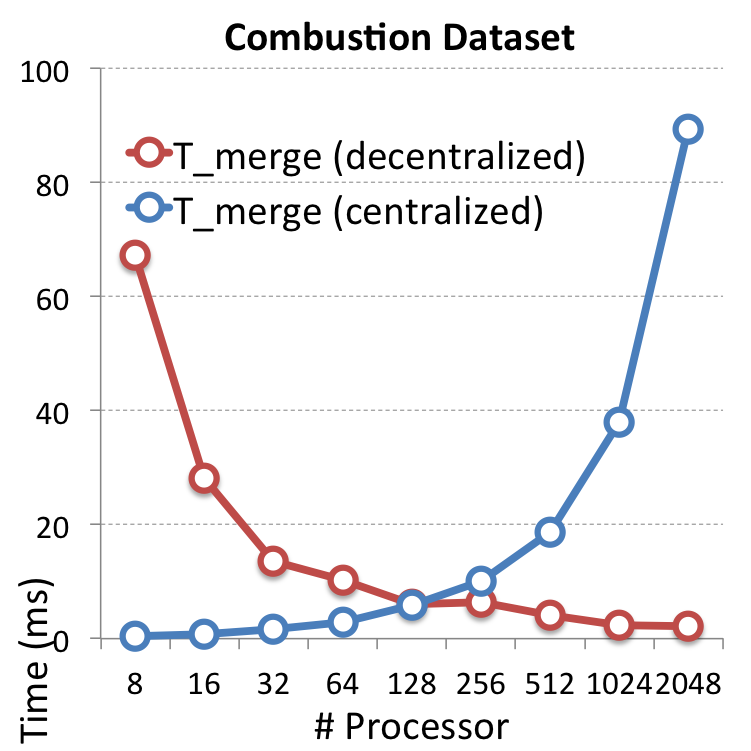
\includegraphics[width=0.45\linewidth]{combustion_local_vs_global.png}
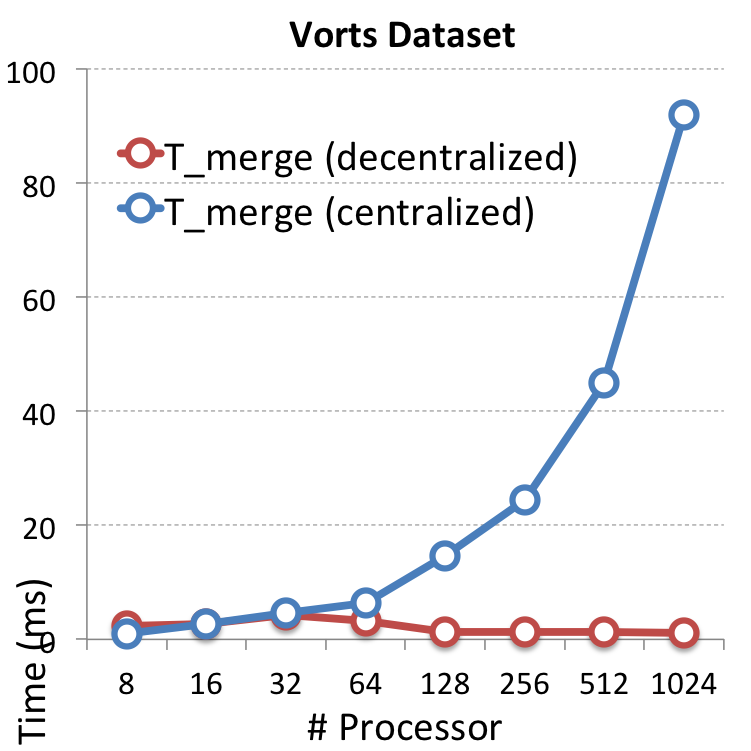
\includegraphics[width=0.45\linewidth]{vorts_local_vs_global.png}
\caption{The comparison of the average computation cost per time step between the centralized and the decentralized approach. The centralized approach works well for a small number of processors while the decentralized approach exceeds after a certain number, e.g. 128 processors for the combustion data set, is used.}
\label{fig:local-vs-global}
\end{figure}

\begin{figure}[t]
\centering
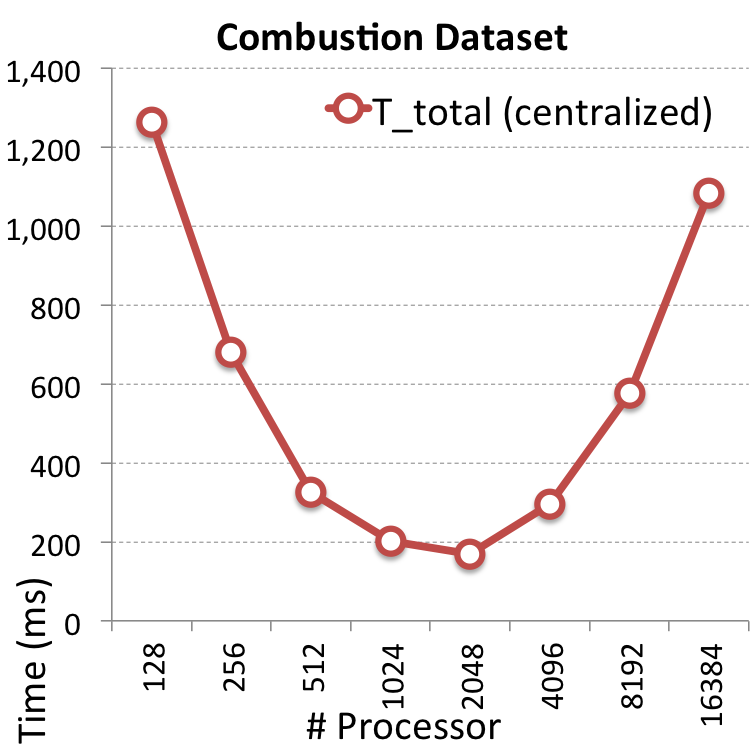
\includegraphics[width=0.49\linewidth]{combustion_t_total_centralized.png}
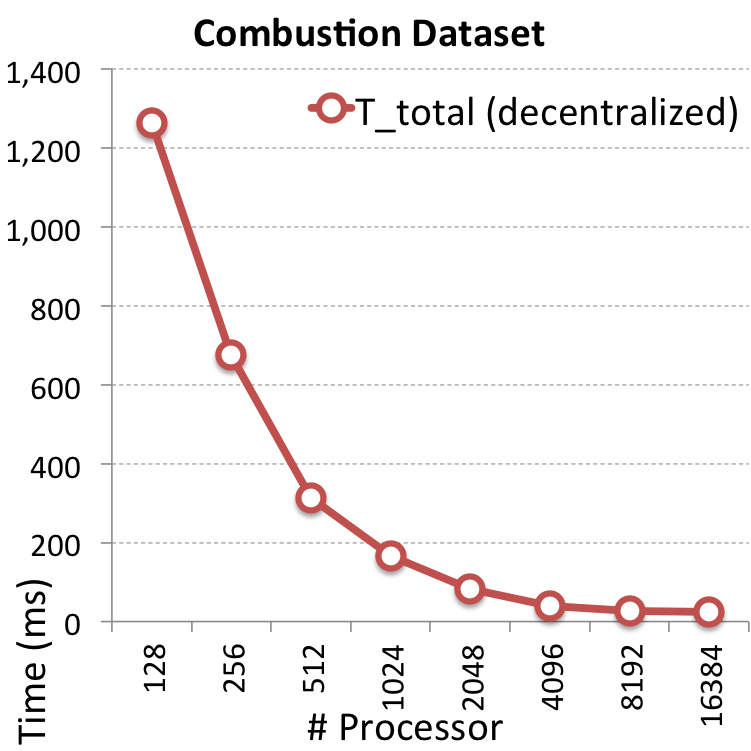
\includegraphics[width=0.49\linewidth]{combustion_t_total_decentralized.png}
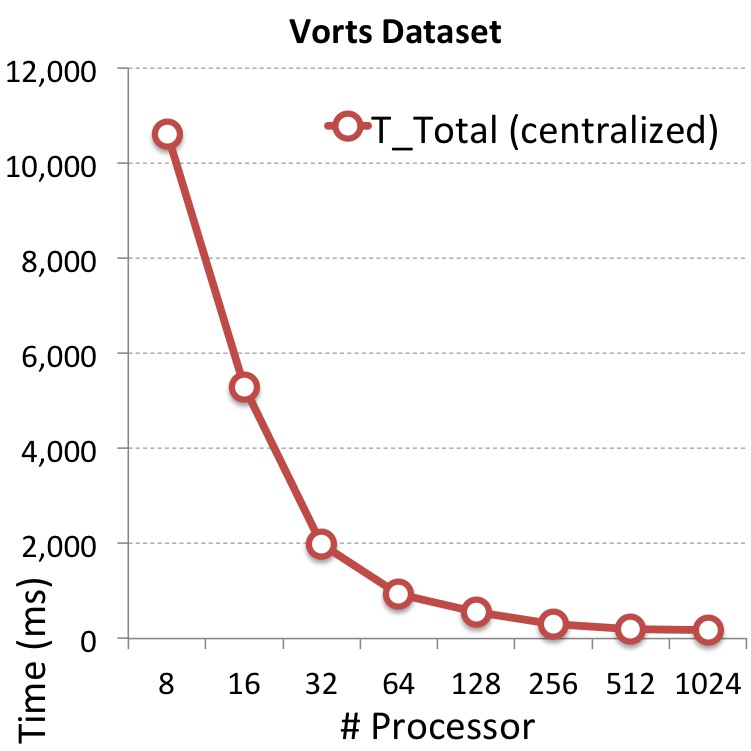
\includegraphics[width=0.49\linewidth]{vorts_t_total_centralized.png}
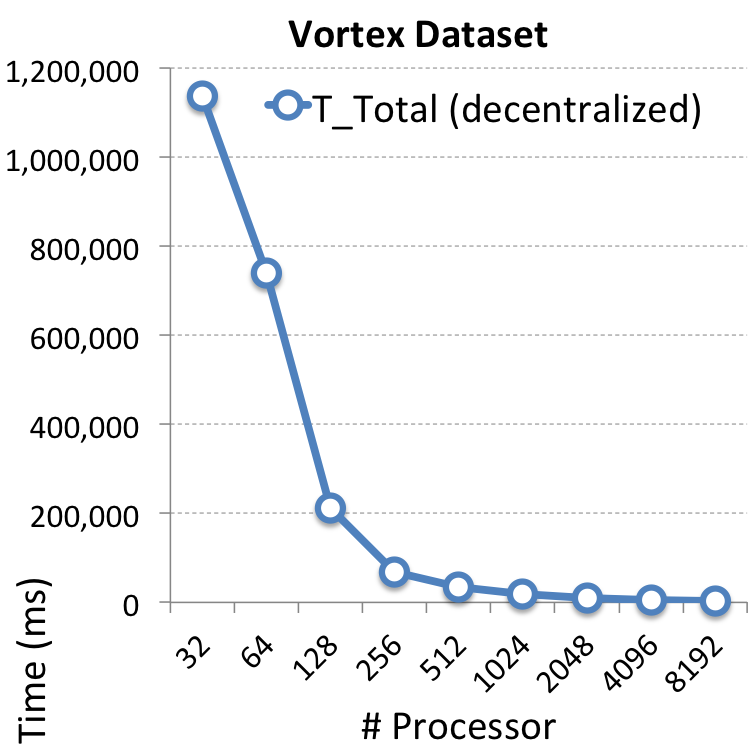
\includegraphics[width=0.49\linewidth]{vorts_t_total_decentralized.png}
\caption{The comparison of the average computation cost per time step for different approaches to global connectivity information generation. The centralized approach scales up to 2048 processors but the merging time outweighs the extraction time when using more processors; The decentralized approach scales linearly up 16384 processors for the combustion data set.}
\label{fig:global-merge}
\end{figure}

\textbf{Create Global Connectivity Information ($T_{merge}$): }
We also compared the performance for both centralized and decentralized approach in creating global connectivity information, which is the major factor related to the scalability of our algorithm. Though the number of features-on-boundary decreases as more processors involve, the communication cost for the centralized approach increases as $N_p$ increases. As shown in Figure~\ref{fig:local-vs-global}, the centralized approach is suitable for scenarios that only a small number of processors are required, while the decentralized approach outperforms when a large amount of processors are used. From the overall performance perspective, when $T_{merge}$ exceeds $T_{extract}$ after using a certain amount of processors, 2048 for instance in Figure~\ref{fig:global-merge}, the overall execution time rebounds for the centralized approach. On the other hand, the decentralized approach scales well up to 16384 processors for the combustion data set, as the communication cost is as low as ${O(\sqrt[3]{N_p})}$.